\subsection{Encoding}
\label{sec:encoders}

\begin{figure*}
    \centering
    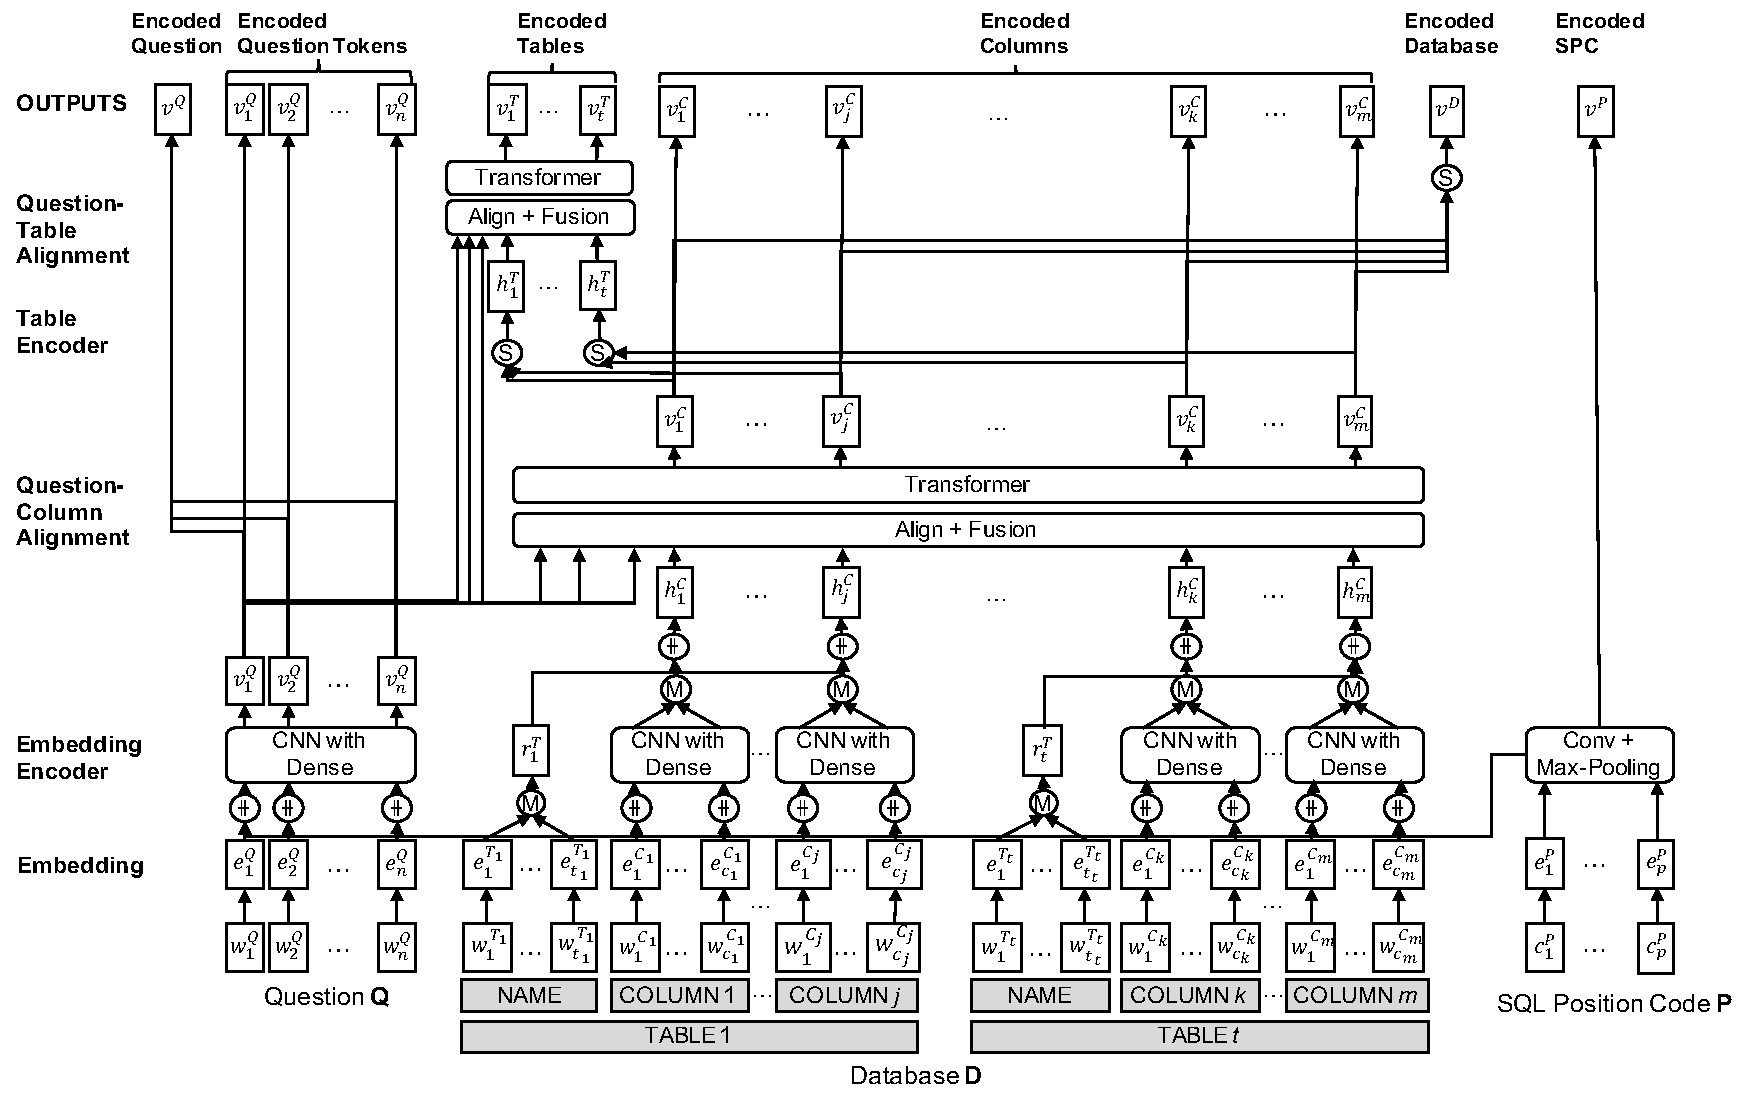
\includegraphics[width=\textwidth]{pics/enc/fig_encode}
    \caption{Network architecture of the proposed input encoder. \raisebox{-0.5ex}{
\includegraphics[height=3.3mm]{pics/enc/mark_1}} represents vector concatenation, \raisebox{-0.5ex}{
\includegraphics[height=3.3mm]{pics/enc/mark_2}} represents max-pooling and \raisebox{-0.5ex}{
\includegraphics[height=3.3mm]{pics/enc/mark_3}} represents self-attention.\cite{choi_ryansql_2020}}
    \label{fig:encode}
\end{figure*}

Encoders\cite{kumar2022deep} are a crucial component in natural language processing tasks and consist of a multi-layered assembly of recurrent elements, such as Long Short-Term Memory (LSTM) units, Gated Recurrent Units (GRUs), or other similar structures. These recurrent elements work in tandem to process an input sequence, with each unit being responsible for handling a single element within the sequence, capturing the pertinent information for that specific element, and subsequently propagating this information forward to the next recurrent unit in the stack.

The primary function of an encoder is to systematically transform textual data into a suitable numerical or vector representation that retains the inherent relationships and dependencies among words, phrases, and sentences\cite{cho-etal-2014-learning}. This is achieved through a combination of techniques, such as tokenization, embedding, and the use of attention mechanisms, which together facilitate the encoding process.

Tokenization serves to break down the input text into smaller, manageable units, such as words or subwords, while embeddings assign a dense vector representation to each token, thus allowing machines to efficiently process and compare these tokens. Attention mechanisms, on the other hand, enable encoders to weigh the importance of different input elements and selectively focus on the most relevant parts of the input sequence when generating the final encoded representation.

By effectively converting the textual data into a machine-understandable format, encoders play a pivotal role in empowering machines to recognize intricate patterns, relationships, and contextual cues within the text. Consequently, this ability to accurately discern the context of sentences and phrases forms the foundation for a wide array of natural language processing tasks, ranging from machine translation and sentiment analysis to text summarization and question-answering systems.

Several approaches have been explored to address the challenges of representing the meaning of questions, capturing the structure of database schemas, and establishing connections between database content and questions in the text-to-SQL domain\cite{deng2022recent}. These methods play a crucial role in facilitating the understanding of the complex relationships between natural language questions and their corresponding SQL queries.

One of the main challenges in text-to-SQL research is effectively representing the meaning of questions. Various encoding methods have been used to capture the semantics of natural language questions, ranging from traditional word embeddings like Word2Vec and GloVe to more advanced contextualized representations like BERT and its variants. These encoding techniques aim to produce meaningful vector representations of questions that models can use to understand and generate accurate SQL queries.

Another important aspect is representing database schemas, which serve as blueprints for organizing and structuring databases. Researchers have used various strategies to encapsulate database schema information, such as graph-based, tree-structured, and sequence-based encodings. These approaches enable text-to-SQL models to understand the hierarchical relationships and dependencies among various database elements. This allows for more accurate and efficient query generation.

Linking database content to questions is a vital task for text-to-SQL systems\cite{deng2022recent}. It involves the identification and mapping of relevant entities and attributes from the question to the database schema. To achieve this, various methods have been employed, including attention mechanisms, entity-linking techniques, and schema-agnostic encodings. These approaches help models identify relevant portions of the database schema and generate SQL queries that accurately reflect the intended meaning of the natural language questions.

Encoding methods and encoders play a crucial role in addressing the challenges of representing question semantics, encapsulating database schema structures, and linking database content to questions in the text-to-SQL domain. The exploration of diverse encoding techniques has led to significant advancements in the development of more accurate and efficient text-to-SQL models, furthering the field's understanding of the complex relationships between natural language questions and SQL queries\cite{deng2022recent}.

\begin{table}
    \centering
    \newcolumntype{g}{>{\columncolor{Gray}}c}
    \begin{tabular}{|c|c|c|c|}
        \hline
        \rowcolor{Gray}
        \textbf{Methods}                & \textbf{Adopted by} & \textbf{Applied datasets} & \textbf{Addressed challenges}                                                                              \\
        \hline

        Encode token type               & TypeSQL             & WikiSQL                   & Representing question meaning                                                                              \\
        \hline
        \multirow{8}{*}{Graph-based}    & GNN                 & Spider                    & \multirow{8}{*}{\parbox{5cm}{Representing question and DB schemas in a structured way and Schema linking}} \\
                                        & Global-GCN          & Spider                    &                                                                                                            \\
                                        & IGSQL               & Sparc, CoSQL              &                                                                                                            \\
                                        & RAT-SQL             & Spider                    &                                                                                                            \\
                                        & LEGSQL              & Spider                    &                                                                                                            \\
                                        & SADGA               & Spider                    &                                                                                                            \\
                                        & ShawdowGNN          & Spider                    &                                                                                                            \\
                                        & S2SQL               & Spider                    &                                                                                                            \\
        \hline
        \multirow{5}{*}{Self-attention} & X-SQL               & WikiSQL                   & \multirow{5}{*}{\parbox{5cm}{Representing question and DB schemas in a structured way and Schema linking}} \\
                                        & SQLova              & WikiSQL                   &                                                                                                            \\
                                        & RAT-SQL             & Spider                    &                                                                                                            \\
                                        & DuoRAT              & Spider                    &                                                                                                            \\
                                        & UnifiedSKG          & WikiSQL, Spider           &                                                                                                            \\
        \hline
        \multirow{4}{*}{Adapt PLM}      & X-SQL               & WikiSQL                   & \multirow{4}{*}{\parbox{5cm}{Leveraging external data to represent question and DB schemas}}               \\
                                        & SQLova              & WikiSQL                   &                                                                                                            \\
                                        & Guo                 & WikiSQL                   &                                                                                                            \\
                                        & HydraNet            & WikiSQL                   &                                                                                                            \\
        \hline
        \multirow{3}{*}{Pre-training}   & TaBERT              & Spider                    & \multirow{3}{*}{\parbox{5cm}{Leveraging external data to represent question and DB schemas}}               \\
                                        & GraPPA              & Spider                    &                                                                                                            \\
                                        & GAP                 & Spider                    &                                                                                                            \\
        \hline
    \end{tabular}
    \caption{Methods used for encoding in text-to-SQL \cite{deng2022recent}}
    \label{tab:methods}
\end{table}

\subsubsection{Encode Token Types}

\subsubsection{Graph-based Methods}

\subsubsection{Self-attention}
\label{sec:methods:encoders:SelfAttention}

Self-attention is a fundamental component in natural language processing (NLP) models, particularly those based on the Transformer architecture. It serves as the primary building block of the transformer structure, as mentioned in the works of X-SQL\cite{he2019xsql}, SQLova\cite{DBLP:journals/corr/abs-1902-01069}, and UnifiedSKG\cite{xie2022unifiedskg}. These models employ the original self-attention mechanism by default.

The self-attention mechanism allows the model to weigh and aggregate different words or tokens in a sequence based on their relative importance\cite{https://doi.org/10.48550/arxiv.1706.03762}. In essence, it helps the model to focus on the most relevant parts of a given input while processing it. This is accomplished by computing attention scores between each pair of tokens in the input, which are then used to produce a weighted sum of the input tokens. The mechanism is particularly effective in handling long-range dependencies within the text.

However, the original self-attention mechanism can be modified to cater to specific tasks or address particular challenges. One such modification is relation-aware self-attention, employed by RAT-SQL\cite{wang_rat_sql_2021} and DuoRAT\cite{scholak-etal-2021-duorat}. This variation of self-attention is designed to take advantage of the relationships between tables and columns when working with structured data.

Relation-aware self-attention extends the original self-attention by incorporating information about the structure and relations in the input data. This additional information is used to adjust the attention scores, allowing the model to focus on the most relevant relationships between different elements in the input. As a result, models equipped with relation-aware self-attention can better handle tasks involving structured data, such as SQL query generation or table-based reasoning.

% \begin{table}[t]
%     \centering
%     \scalebox{0.8}{
%         \begin{tabular}{lcc}
%             \toprule
%             \textbf{Model}                                 & \textbf{EMA Dev.} \\
%             \midrule
%             X-SQL\cite{he2019xsql}                         & 89.5              \\
%             SQLova\cite{DBLP:journals/corr/abs-1902-01069} & 87.2              \\
%             RATSQL \cite{wang_rat_sql_2021}                & 69.7              \\
%             UnifiedSKG\cite{xie2022unifiedskg}             & 72.3              \\
%             DuoRAT\cite{scholak-etal-2021-duorat}          & 75.1              \\
%             \bottomrule
%         \end{tabular}
%     }
%     \caption{The exact match accuracy on the Spider dev set.}
%     \label{table:methods:encoders:SelfAttention}
% \end{table}
\subsubsection{Adapt PLM} %Pre-trained Language Models
\label{sec:adaptplm}

\begin{figure*}[htbp]
    \centering
    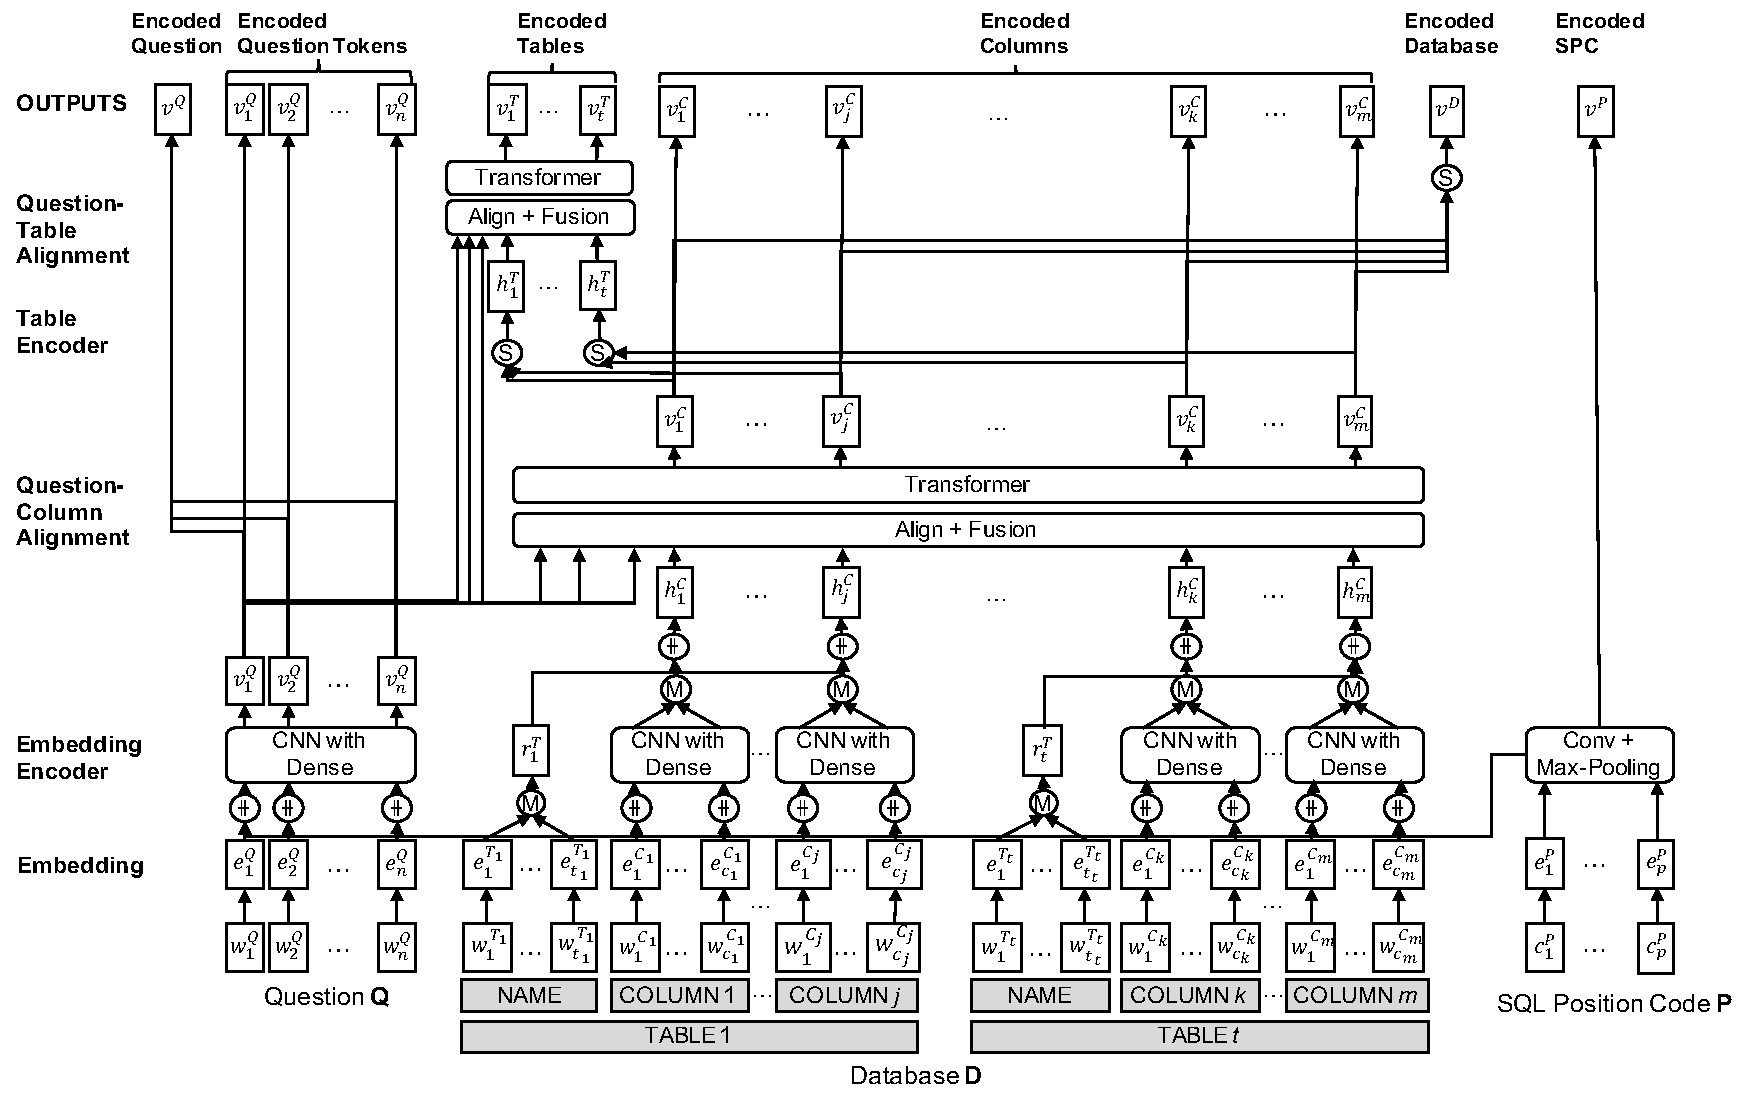
\includegraphics[width=\textwidth]{pics/enc/fig_encode}
    \caption{Network architecture of the proposed input encoder. \raisebox{-0.5ex}{
\includegraphics[height=3.3mm]{pics/enc/mark_1}} represents vector concatenation, \raisebox{-0.5ex}{
\includegraphics[height=3.3mm]{pics/enc/mark_2}} represents max-pooling and \raisebox{-0.5ex}{
\includegraphics[height=3.3mm]{pics/enc/mark_3}} represents self-attention.\cite{choi_ryansql_2020}}
    \label{fig:ryan}
\end{figure*}

Adapt \ac{PLM} methods aim to utilize the knowledge encapsulated in pre-trained language models, such as BERT\cite{DBLP:journals/corr/abs-1810-04805}, to improve their performance on text-to-SQL tasks. These methods modify or extend the original PLMs to better align with the specific requirements of the task.

One common approach is to encode both the natural language questions and the database schemas using PLMs. For instance, SQLova\cite{DBLP:journals/corr/abs-1902-01069} and RYANSQL\cite{10.1162/coli_a_00403} concatenate the question words and schema words as input to the BERT encoder. This approach allows the model to learn representations that capture the relationships between questions and the underlying schema. In figure \ref{fig:ryan}, the authors of RYANSQL\cite{10.1162/coli_a_00403} propose a novel encoder that combines the BERT encoder with a self-attention mechanism to capture the interactions between the question and schema words. As you can see it passes the question words and database tables schemas through embedding layers, then concatenates them and passes them through the BERT encoder. The output of the BERT encoder is then passed through a self-attention layer to capture the interactions between the question and schema words. The self-attention layer is then concatenated with the BERT encoder output and passed through a feed-forward network to produce the final representation of the question and schema.

Some methods go a step further by adjusting the embeddings produced by the PLMs. X-SQL\cite{he2019xsql} proposes the replacement of the segment embeddings from the pre-trained encoder with column-type embeddings for the WikiSQL dataset. Guo and Gao \cite{guo2020content} introduce an approach that encodes additional feature vectors for matching between question tokens and table cells, as well as column names. These feature vectors are then concatenated with the BERT embeddings of questions and DB schemas.

HydraNet\cite{lyu_hybrid_2020} uses BERT to encode the question and individual columns, an approach that is more aligned with the tasks BERT is pre-trained on. After obtaining BERT representations for all columns, the model selects the top-ranked columns for SQL prediction


\begin{table}[t]
    \centering
    \scalebox{0.8}{
        \begin{tabular}{lcc}
            \toprule
            \textbf{Model}                                  & \textbf{Execution Accuracy} \\
            Seq2SQL\cite{zhong_seq2sql_2017}                & 60.8                        \\
            TypeSQL\cite{DBLP:journals/corr/abs-1804-09769} & 74.5                        \\
            \midrule
            SQLova\cite{DBLP:journals/corr/abs-1902-01069}  & 90.2                        \\
            Guo\cite{guo2020content}                        & 91.1                        \\
            HydraNet\cite{lyu_hybrid_2020}                  & 92.4                        \\
            \bottomrule
        \end{tabular}
    }
    \caption{The execution accuracy on the WikiSQL dev set.}
    \label{table:methods:encoders:adaptplm}
\end{table}

Examining the WikiSQL benchmark results in Table \ref{table:methods:encoders:adaptplm}, we can observe a significant overall performance improvement when employing pre-trained language models (PLMs) compared to previous methods. This enhancement can be attributed to the ability of PLMs, such as BERT, to capture complex linguistic patterns and relationships within the input data. By leveraging the knowledge encapsulated in these models and adapting them to the text-to-SQL task, researchers have been able to achieve better alignment with the specific requirements of the problem domain. As a result, PLM-based approaches have demonstrated superior performance in generating accurate SQL queries from natural language questions, surpassing traditional methods and showcasing the potential of PLMs in addressing complex language understanding tasks.

\subsubsection{Pre-training}


